\documentclass{book}

\usepackage{amssymb}
\usepackage{amsmath}
\usepackage{amsthm}
\usepackage{arydshln}
\usepackage{calc}
\usepackage{cancel}
\usepackage{caption}
\usepackage{cite}
\usepackage{color}
\usepackage{enumitem}
\usepackage{esint}
\usepackage{etoolbox}
\usepackage{float}
\usepackage{framed}
\usepackage{fullpage}
\usepackage{gensymb}
\usepackage[margin=1in]{geometry}
\usepackage{graphicx}
\usepackage{listings}
\usepackage{multirow}
\usepackage{subfiles}
\usepackage{rsfso}
\usepackage{tikz}
\usepackage{tikz-3dplot}
\usepackage{ushort}
\usepackage{wrapfig}
\usepackage{xcolor}
\usepackage{soul}
\usepackage{epstopdf}

% pdf versions
\pdfoptionpdfminorversion=7

% handle page stretching
\raggedbottom

% Graphics file location
\graphicspath{{Graphics/}{../Graphics/}}

% Use for drawings
\usetikzlibrary{angles,arrows,calc,decorations,intersections,patterns,positioning,quotes,shapes}
\usetikzlibrary{shapes.geometric}
\usetikzlibrary{decorations.pathreplacing}
\newcommand{\midarrow}{\tikz \draw[-latex] (0,0) -- +(.1,0);}

% Tikz commands for drawing block diagrams, etc...
\tikzset{%
	block/.style    = {draw, rectangle, minimum height = 2em, minimum width = 2em},
	sum/.style      = {draw, circle}, % Adder
	input/.style    = {fill=white, rectangle}, % Input
	output/.style   = {fill=white, rectangle}, % Output
	waypoint/.style   = {coordinate}, % Output
}

\tikzset{%
	startstop/.style= {draw, rectangle, rounded corners, minimum width=2cm, minimum height=1cm,text centered},
	inout/.style    = {draw, trapezium, trapezium left angle=70, trapezium right angle=110, minimum width=2cm, minimum height=1cm, text centered},
	process/.style  = {draw, rectangle, minimum width=2cm, minimum height=1cm, text centered},
	decision/.style = {draw, diamond, minimum width=1.5cm, minimum height=1cm, text centered, diamond, aspect=2},
	arrow/.style    = {thick,-latex,>=stealth},		
}

\tikzset{
	saveuse path/.code 2 args={
		\pgfkeysalso{#1/.style={insert path={#2}}}%
		\global\expandafter\let\csname pgfk@\pgfkeyscurrentpath/.@cmd\expandafter\endcsname
		% not optimal as it is now global through out the document
		\csname pgfk@\pgfkeyscurrentpath/.@cmd\endcsname
		\pgfkeysalso{#1}},
	/pgf/math set seed/.code=\pgfmathsetseed{#1}}

% Define Laplace, Fourier transform symbols
\newcommand{\LT}{\mathcal{L}}
\newcommand{\FT}{\mathcal{F}}

% Define adjugate function
\newcommand{\adj}{\text{adj}}

% Define rank function
\newcommand{\rank}{\text{rank}}

% commands to speed up writing j\omega and s-plane
\newcommand{\jw}{j\omega}
\newcommand{\jt}{j\theta}
\newcommand{\wt}{\omega t}
\newcommand{\zw}{\zeta\omega_n}
\newcommand{\spl}{s\textrm{-plane}}
\newcommand{\Lm}{\textrm{Lm }}
% Clean up overline/underline for math mode
\def\obar#1{\bar{#1}}
\def\ubar#1{\ushort{#1}}

\newcommand{\exmp}{\subsubsection*{Example}}
\newcommand{\nib}{\noindent$ \bullet\ $}


\begin{document}
\chapter*{Lecture 7}
Last time: Response of 2nd order systems:
\begin{itemize}
	\item Underdamped Response
	\item Performance Metrics
	\begin{itemize}
		\item Peak time $ t_p $
		\item Rise time $ t_r $
		\item Settling time $ t_s $
		\item Overshoot Percent $ \%OS $
	\end{itemize}
	\item 2nd order systems with a zero and 3rd and higher order systems
	\begin{itemize}
		\item Same formulae can be used if the extra poles/zeros are far removed from the dominant 2nd order poles (far removed: 4 to 5 times further left of the $ \jw $-axis).
	\end{itemize}
\end{itemize}
Note that we have not as of yet addressed the issue of accuracy of the final value of a system's output, in other words how close a system's final value is to the desired value. Another name for this is \textbf{steady-state error}. We will take care of a few other matters first, and then we will return to tack this problem later.

\section*{Stability}
What is stability? Per the Webster Dictionary: ``Stability is the property of a body that causes it when disturbed from a condition of equilibrium or steady motion to develop forces or moments that restore the original condition.'' This kind of stability is for small perturbations to the system.
%What is stability? It has to do with whether or not the output (response) of a system ``blows up''. (Note: we can always get a system to ``blow up'', depending on what we put into it, e.g. an unbounded input) There is a difference between the way ``stability'' is defined in classical dynamics and the way it is viewed in control theory. In classical dynamics, stability decision is based upon the response to initial conditions.
\begin{center}
	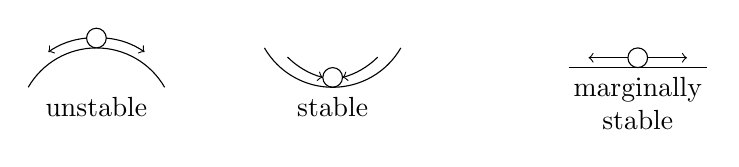
\begin{tikzpicture}
	\draw (0,0.5) arc (90:30:1);
	\draw (0,0.5) arc (90:150:1);
	\draw[->] (0.125,0.625) arc (85:55:1);
	\draw[->] (-0.125,0.625) arc (95:125:1);
	\draw (0,0.625) circle (0.125);
	\node[below] at (0,0) {unstable};
	
	\draw (3,0) arc (270:330:1);
	\draw (3,0) arc (270:210:1);
	\draw[<-] (2.875,0.125) arc (255:225:1);
	\draw[<-] (3.125,0.125) arc (285:315:1);
	\draw (3,0.125) circle (0.125);
	\node[below] at (3,0) {stable};
	
	\draw (6,0.25) -- (7.75,0.25);
	\draw[->] (6.75,0.375) -- (6.25,.375);
	\draw[->] (7.00,0.375) -- (7.5,.375);
	\draw (6.875,0.375) circle (0.125);
	\node[below,align=center] at (6.875,0.25) {marginally\\stable};
	\end{tikzpicture}
\end{center}
In controls: A system is stable if all bounded inputs to the system produce bounded outputs; the system is unstable otherwise. This is called \textbf{Bounded-Input Bounded-Output} (BIBO) stability.

Let's look at things from the perspective of poles and zeros.
\[ Y(s)=G(s)U(s) \]
So, the nature of the system output $ y(t) $ depends on
\begin{itemize}
	\item the poles of $ G(s) $
	\item the poles of $ U(s) $
\end{itemize}
Since $ u(t) $ needs to be bounded, poles of $ U(s) $ can include poles located:
\begin{itemize}
	\item Strictly in the LHP
	\item At the origin (at most 1)
	\item On the $ \jw $-axis as a complex conjugate pair (there can be any number of these, so long as they are not repeated).
\end{itemize}
So, the requirements on poles of $ G(s) $ for BIBO stability are:
\begin{itemize}
	\item They must \textbf{all} be strictly in the LHP. Otherwise, it would be possible to find a bounded input that will result in an unbounded output.
	\begin{itemize}
		\item Roots of denominator of $ G(s) $ must all have strictly negative real parts.
	\end{itemize}
	\item The system is BIBO unstable if $ G(s) $ possesses poles in the RHP or on the imaginary axis.
\end{itemize}
So, we can look at the pole-zero pattern of a system's transfer function, and tell whether the system is BIBO stable or not.

\exmp
\begin{center}
	\begin{tabular}{c c c}
		$ G(s) = \dfrac{1}{(s+1)(s+2)} $ & $ \longleftarrow $ & BIBO stable \\
		$ G(s) = \dfrac{1}{s} $ & $ \longleftarrow $ & BIBO unstable \\
		$ G(s) = \dfrac{\omega}{s^2+\omega^2} $ & $ \longleftarrow $ & BIBO unstable \\
		$ G(s) = \dfrac{2-s}{(s+1)(s+2)(s+3)} $ & $ \longleftarrow $ & BIBO stable \\
		$ G(s) = \dfrac{1}{(s+1)(s-2)(s+3)} $ & $ \longleftarrow $ & BIBO unstable \\
	\end{tabular}
\end{center}
This is all easy if the denominator of $ G(s) $ is given in factored form. But what if the denominator is not factored?
\begin{itemize}
	\item[a)] Use a calculator or Matlab to factor. This works only if you have numbers for the denominator coefficients.
	\item[b)] Use a method that does not factor the denominator explicitly, but tells you how many of its roots are in the LHP, RHP and $ \jw $-axis (stability information). This is good when the coefficients of the denominator polynomials are either numbers \textbf{or} symbols.
\end{itemize}

\subsection*{Tests for Stability}
Given the denominator polynomial, $ p(s) $, of a transfer function
\[ p(s) = a_ns^n + a_{n-1}s^{n-1} + \ldots + a_1s + a_0 \]
determine whether there are roots of $ p(s) $ with positive real parts (RHP), or no real parts ($ \jw $-axis).

\paragraph{Test \#1:} This test comes from the mathematics of polynomials. Check the coefficients $ a_k $. If any are missing or if any two $ a_k $ have opposite sign, then there is a zero of $ p(s) $ on the imaginary axis or in the RHP. If this is the case, then the system is clearly BIBO unstable. 

\exmp
\[ p(s) = s-4 \quad\Rightarrow\quad a_1=1,\ a_0 = -4. \text{ Sign change, therefore unstable.}\]
\[ p(s) = s^2+9 \quad\Rightarrow\quad a_2=1,\ a_1=0,\ a_0 = 9. \text{ $ a_1 = 0 $, therefore unstable.}\]

This test is necessary to determine stability, but it is not sufficient. A system can satisfy this test and still be unstable!

\paragraph*{Test \#2:} Routh-Hurwitz Criterion. Construct the \textbf{Routh Array} and examine the 1st column. The number of zeros of $ p(s) $ in the RHP is the number of sign changes in the 1st column of the Routh array.

Basic rules for constructing the Routh array: Let $ p(s) $ be:
\[ p(s) = a_ns^n + a_{n-1}s^{n-1} + \ldots + a_1s + a_0 \]
\begin{minipage}[t]{0.30\textwidth}
	\begin{center}
		\textbf{Rules:}
	\end{center}
	\begin{itemize}[leftmargin=*]
	\item The 1st two \textbf{rows} of the Routh array are constructed with the $ a_k $ coefficients. 
	This means you will have $ (n+1)/2 $ (rounded up) \textbf{columns} in the Routh array.
	\item You will eventually have $ n+1 $ \textbf{rows} in the Routh array. To calculate an element of the array, form a $ 2\times2 $ matrix, denoted $ A $, using the preceding two rows' 1st column and column to the immediate right of the element you want to determine. The element is $ = -(\det A)/A_{21} $. 
	\end{itemize} 
\end{minipage}
\begin{minipage}[t]{0.34\textwidth}
	\centering
	\textbf{Array:}
	\vspace{1em}
	
	\begin{tabular}{|c|c|c|c|}\hline
		&  &  &  \\ 
		$ a_n $ & $ a_{n-2} $ & $ a_{n-4} $ & $ \ \ldots\ $ \\ 
		&  &  &  \\ \hline
		&  &  &  \\ 
		$ a_{n-1} $ & $ a_{n-3} $ & $ a_{n-5} $ & $ \ \ldots\ $ \\
		&  &  &  \\ \hline
		&  &  &  \\ 
		$ b_1 $ & $ b_2 $ & $ b_3 $ & $ \ \ldots\ $ \\
		&  &  &  \\ \hline
		&  &  &  \\ 
		$ c_1 $ & $ c_2 $ & $ c_3 $ & $ \ \ldots\ $ \\
		&  &  &  \\ \hline
		&  &  &  \\ 
		$ \vdots $ & $ \vdots $ & $ \vdots $ & $ \ \ddots\ $ \\
		&  &  &  \\ \hline
	\end{tabular}
\end{minipage}
\begin{minipage}[t]{0.35\textwidth}\centering
	\textbf{Equations:}
	\small
	\begin{align*}
	b_i &= \dfrac{-\left|\begin{array}{c c} a_n & a_{n-2i} \\ a_{n-1} & a_{n-(2i+1)} \end{array}\right|}{a_{n-1}} \\ 
	& = \frac{(a_{n-1}\times a_{n-2i}) - (a_{n}\times a_{n-(2i+1)})}{a_{n-1}}
	\end{align*}\vspace{-1.5em}
	\begin{align*}
	c_i &= \dfrac{-\left|\begin{array}{c c} a_{n-1} & a_{n-(2i+1)} \\ b_{1} & b_{i+1} \end{array}\right|}{b_{1}} \\
	& = \frac{(b_1\times a_{n-(2i+1)}) - (a_{n-1}\times b_{i+1})}{b_1}
	\end{align*}\vspace{-1.5em}
	\begin{align*}
	d_i &= \dfrac{-\left|\begin{array}{c c} b_{1} & b_{i+1} \\ c_{1} & c_{i+1} \end{array}\right|}{b_{1}} \\
	&= \frac{(c_1\times b_{i+1}) - (c_{i+1}\times b_{1})}{c_1}
	\end{align*}\vspace{-1.5em}
	\[ \text{etc}\ldots \]
\end{minipage}\vspace{1em}

When completed, the number of sign changes in the 1st column of the Routh array is the number of poles in the RHP. \vspace{1em}

For example,
\[ p(s) = a_4s^4 + a_3s^3 + a_2s^2 + a_1s + a_0 \]
\begin{center}
	\begin{minipage}{0.4\textwidth}
		\centering
		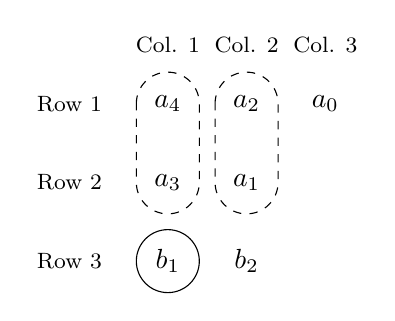
\begin{tikzpicture}[node distance = 1cm]
		\node (an) {$ a_4 $};
		\node[below of=an] (an1) {$ a_{3} $};
		\node[right of=an] (an2) {$ a_{2} $};
		\node[right of=an1] (an3) {$ a_{1} $};
		\node[right of=an2] (an4) {$ a_{0} $};
		\node[below of=an1] (b1) {$ b_1 $};
		\node[below of=an3] (b2) {$ b_2 $};
		\draw[dashed] (-0.4cm,0) arc (180:0:0.4cm) -- ++(0,-1cm) arc (360:180:0.4cm) -- ++(0,1cm);
		\draw[dashed] (1cm-0.4cm,0) arc (180:0:0.4cm) -- ++(0,-1cm) arc (360:180:0.4cm) -- ++(0,1cm);
		\draw (0,-2cm) circle (0.4cm);
		
		\node[left of=an,node distance=1.25cm] {\footnotesize Row 1};
		\node[left of=an1,node distance=1.25cm] {\footnotesize Row 2};
		\node[left of=b1,node distance=1.25cm] {\footnotesize Row 3};
		\node[above of=an,node distance=0.75cm] {\footnotesize Col. 1};
		\node[above of=an2,node distance=0.75cm] {\footnotesize Col. 2};
		\node[above of=an4,node distance=0.75cm] {\footnotesize Col. 3};
		\end{tikzpicture}
		\[ b_1 = -\frac{\left|\begin{array}{c c}	a_4 & a_2 \\ a_3 & a_1 \end{array}\right|}{a_3} = \frac{a_2a_3 - a_4a_1 }{a_3} \]
	\end{minipage}
	\begin{minipage}{0.4\textwidth}
		\centering
		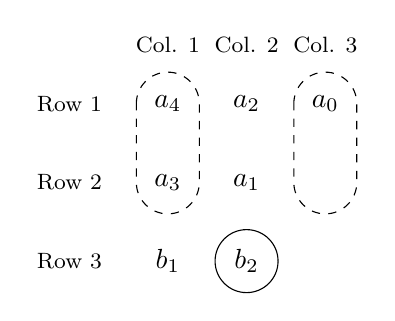
\begin{tikzpicture}[node distance = 1cm]
		\node (an) {$ a_4 $};
		\node[below of=an] (an1) {$ a_{3} $};
		\node[right of=an] (an2) {$ a_{2} $};
		\node[right of=an1] (an3) {$ a_{1} $};
		\node[right of=an2] (an4) {$ a_{0} $};
		\node[below of=an1] (b1) {$ b_1 $};
		\node[below of=an3] (b2) {$ b_2 $};
		\draw[dashed] (-0.4cm,0) arc (180:0:0.4cm) -- ++(0,-1cm) arc (360:180:0.4cm) -- ++(0,1cm);
		\draw[dashed] (2cm-0.4cm,0) arc (180:0:0.4cm) -- ++(0,-1cm) arc (360:180:0.4cm) -- ++(0,1cm);
		\draw (1cm,-2cm) circle (0.4cm);
		
		\node[left of=an,node distance=1.25cm] {\footnotesize Row 1};
		\node[left of=an1,node distance=1.25cm] {\footnotesize Row 2};
		\node[left of=b1,node distance=1.25cm] {\footnotesize Row 3};
		\node[above of=an,node distance=0.75cm] {\footnotesize Col. 1};
		\node[above of=an2,node distance=0.75cm] {\footnotesize Col. 2};
		\node[above of=an4,node distance=0.75cm] {\footnotesize Col. 3};
		\end{tikzpicture}
		\[ b_2 = -\frac{\left|\begin{array}{c c}	a_4 & a_0 \\ a_3 & 0 \end{array}\right|}{a_3} = \frac{a_0a_3}{a_3} \]
	\end{minipage}
\end{center}

Let's do some examples of using Routh-Hurwitz to determine stability. One way to keep track of the number of rows needed is to label the rows: $ s^n $, $ s^{n-1} $, $ \ldots $, $ s^0 $. So, a third order polynomial will have rows labeled $ s^3,\ s^2,\ s,\ s^0 $ (4 rows).
\exmp
Consider a system with the following denominator polynomial function:
\[ p(s) = s^3 + 4s^2 + 3s + 2 \]
Determine stability using a Routh array.
\begin{center}
	\begin{tabular}{c c c c} \vspace{1em}
		$ s^3 $: & 1 & 3 & 0 \\ \vspace{1em}
		$ s^2 $: & 4 & 2 & 0 \\ \vspace{1em}
		$ s^1 $: & $ -\frac{2-12}{4} = \frac{5}{2} $ & $ -\frac{1\cdot0-0\cdot4}{4}=0 $ &  \\ \vspace{1em}
		$ s^0 $: & $ -\frac{2}{5} \left(4\cdot0 - 2\cdot \frac{5}{2}\right) = 2 $ & 0 & \\
	\end{tabular}
\end{center}
There are no sign changes in the first column, so the system is stable.

\exmp
Consider a system with the following denominator polynomial function:
\[ p(s) = s^3 + 4s^2 + 3s + 13 \]
Determine stability using a Routh array.
\begin{center}
	\begin{tabular}{c c c} \vspace{1em}
		$ s^3 $: & 	1 & 3 \\ \vspace{1em}
		$ s^2 $: & 	4 & 13 \\ \vspace{1em}
		$ s^1 $: & 	$ - \frac{13-12}{4} = -\frac{1}{4} $ & \\ \vspace{1em}
		$ s^0 $: & 	$ \frac{-1}{-1/4} \left(4\cdot0 + 13\cdot \frac{1}{4}\right) = 13 $ & \\
	\end{tabular}
\end{center}

There are \textbf{two} sign changes in the first column, so the system has two RHP poles and is unstable.

\exmp
It is OK to multiply an entire row by a constant; this does not change what happens in the succeeding rows, and helps simplify the math. Consider a system with the following denominator polynomial function:
\[ p(s) = s^4 + 10s^3 + 35s^2 + 50s + 24 \]
Determine stability using a Routh array.
\begin{center}
	\begin{tabular}{c c c c l}\vspace{1em}
		$ s^4 $: &  1 & 35 & 24 & \\ \vspace{1em}
		$ s^3 $: & $ \cancel{10}^{\ 1} $ & $ \cancel{50}^{\ 5} $ & 0 & multiply row by 1/10 \\ \vspace{1em}
		$ s^2 $: & $ \frac{35-5}{1}=\cancel{30}^{\ 5} $ & $ \frac{24-0}{1}=\cancel{24}^{\ 4}$ &0 & find $ b_1=30 $ and $ b_2=24 $ , then multiply by 1/6\\ \vspace{1em}
		$ s^1 $: & $ \frac{25-4}{5}=\frac{21}{5} $ &0 & & \\ \vspace{1em}
		$ s^0 $: & $ \frac{5}{21}\cdot\left(\frac{21}{5}\cdot4-0\right) = 4 $ &0 & &
	\end{tabular}
\end{center}
There are no sign changes in the first column, so the system is stable. 

\exmp
Consider a system with the following denominator polynomial function:
\[ p(s) = s^4 + 3s^3 + 3s^2 + 12s + 8 \]
Determine stability using a Routh array.
\begin{center}
	\begin{tabular}{c c c c l}\vspace{1em}
		$ s^4 $: &  1 & 3 & 8 & \\ \vspace{1em}
		$ s^3 $: & 3 & 12 & 0 & \\ \vspace{1em}
		$ s^2 $: & $ -\frac{12-9}{3}=-1 $ & $ \frac{24-0}{3}=8$ & 0 & \\ \vspace{1em}
		$ s^1 $: & $ -\frac{24+12}{-1}=36 $ & 0& & \\ \vspace{1em}
		$ s^0 $: & $ \frac{36\cdot 8 - 0}{36} = 8 $ &0 & &
	\end{tabular}
\end{center}
There are two sign changes in the first column, so the system is unstable with two poles in the RHP. 

\subsection*{Variables in the Routh Array}
Routh-Hurwitz is particularly useful for determining stability for systems with variables as coefficients.
\exmp
Consider a system with the following denominator polynomial function:
\[ p(s) = s^3 + 2s^2 + 4s + (3+K) \]
For what range of $ K $ will the system be stable?
\begin{center}
	\begin{tabular}{c c c c l}\vspace{1em}
		$ s^3 $: &  1 & 4 & 0 & \\ \vspace{1em}
		$ s^2 $: & 2 & 3+K & 0 & \\ \vspace{1em}
		$ s^1 $: & $ b_1=\frac{8-3-K}{2}=\frac{5-K}{2} $ & 0 & 0 & \\ \vspace{1em}
		$ s^0 $: & $ c_1=\frac{2}{5-K}\cdot\left(\frac{5-K}{2}\cdot(3+K)-0\right) = 3+K $ & 0& &
	\end{tabular}
\end{center}
So, for the system to be stable we need
\[ \frac{5-K}{2} > 0 \quad\Rightarrow\quad K<5 \]
\[ 3+K > 0 \quad\Rightarrow\quad K>-3 \]
Therefore the system is stable for $ -3<K<5 $

\subsection*{0-elements in the 1st Column of the Routh Array}
How do we approach a system where we get 0 in the first column of the Routh array? This would require dividing by zero. The $ \epsilon $-method involves replacing the 0 with a value $ \epsilon $, proceeding with the Routh array, and then bring $ \epsilon $ back to 0 once all elements of the Routh array have been determined.
\exmp
Consider a system with the following denominator polynomial function:
\[ p(s) = s^4 + 2s^3 + s^2 + 2s + 5 \]
\begin{center}
	\begin{tabular}{c c c c l}\vspace{1em}
		$ s^4 $: &  1 & 1 & 5 & \\ \vspace{1em}
		$ s^3 $: & 2 & 2 & 0 & \\ \vspace{1em}
		$ s^2 $: & $ -\frac{2-2}{2}=\cancel{0}^{\ \epsilon} $ & $ -\frac{0-10}{2}=5 $ & 0 &  Imagine that the zero is some small value $ \epsilon $ \\ \vspace{1em}
		$ s^1 $: & $ \frac{2\epsilon-10}{\epsilon} $ & 0& &\\ \vspace{1em}
		$ s^0 $: &  $ \frac{10\epsilon -50}{\epsilon}\cdot\frac{\epsilon}{2\epsilon-10} = 5$
	\end{tabular}
\end{center}
So, the first column has elements 
\[ 1,\ 2,\ \epsilon,\ \frac{2\epsilon-10}{\epsilon},\ 5 \]
Stability depends on the $ \epsilon $ and $ \frac{2\epsilon-10}{\epsilon} $ terms. What happens as we bring $ \epsilon $ back to 0? If we start with negative $ \epsilon $, then we know the system is unstable because $ \epsilon $ is an element of the first column. If we start with positive $ \epsilon $ and approach zero from the right, then
\[ \lim_{\epsilon\to0^+} \frac{2\epsilon-10}{\epsilon} = -\infty \]
So, the system is unstable and has two unstable poles.

\subsection*{Row of 0-elements in the Routh Array}
How do we approach a system where an entire row is filled with zeros? This implies that an even number of poles of the system are arranged symmetrically around the origin. \textbf{This is in fact the only way to have poles on the $ \jw $ axis}.
\begin{center}
	\begin{tikzpicture}
	\draw (-2,0) -- (2,0) node[below left] {$ \sigma $};
	\draw (0,-2) -- (0,2) node[below left] {$ j\omega $};
	\node at (-1.25,0) {\Large$ \times $};
	\node at (1.25,0) {\Large$ \times $};
	\node at (0,-1.25) {\Large$ \times $};
	\node at (0,1.25) {\Large$ \times $};
	\node at (-1.25*0.707,1.25*0.707) {\Large$ \times $};
	\node at (1.25*0.707,1.25*0.707) {\Large$ \times $};
	\node at (-1.25*0.707,-1.25*0.707) {\Large$ \times $};
	\node at (1.25*0.707,-1.25*0.707) {\Large$ \times $};
	\end{tikzpicture}
\end{center}
This implies that either there are poles in the RHP and/or there are poles on the $ j\omega $-axis. \textbf{Therefore, the system is BIBO unstable}. This is the only situation that will yield poles on the imaginary axis. There is a way to determine how many of the poles (roots) are on the imaginary axis and how many are in the RHP. We will demonstrate this with an example.

\exmp
Consider a system with the following transfer function:
\[ G(s) = \frac{507s}{s^5 + 3s^4 + 10s^3 + 30s^2 + 169s + 507} \]
And therefore the following denominator polynomial function:
\[ p(s) = s^5 + 3s^4 + 10s^3 + 30s^2 + 169s + 507 \]
\begin{center}
	\begin{tabular}{c c c c l}\vspace{1em}
		$ s^5 $: &  1 & 10 & 169 & \\ \vspace{1em}
		$ s^4 $: & $ \cancel{3}^{\ 1} $ & $ \cancel{30}^{\ 10} $ & $ \cancel{507}^{\ 169} $ & Divide row by 3. \\ \vspace{1em}
		$ s^3 $: & $ \frac{10-10}{1}=0 $ & $ \frac{169-169}{10}=0 $ & 0 &  Entire row is zeros! \\ \vspace{1em}
		$ s^1 $: & $ \cdots $ & & &
	\end{tabular}
\end{center}
Given the row of zeros, we cannot proceed. The approach around this is to use an auxiliary polynomial, formed from the coefficients of the prior row.
\[ P_{aux}(s) = s^4 + 10s^2 + 169 \]
We differentiate this polynomial with respect to $ s $ and obtain
\[ \frac{dP_{aux}}{ds}(s) = 4s^3 + 20s + 0 \]
Then, we replace the row of zeros with the coefficients of this new polynomial (we will divide this row through by 4 to simplify the later math). We can then continue with the standard procedure.
\begin{center}
	\begin{tabular}{c c c c l}\vspace{1em}
		$ s^5 $: &  1 & 10 & 169 & \\ \vspace{1em}
		$ s^4 $: & 1 & 10 & 169 & \\ \vspace{1em}
		$ s^3 $: & $ \cancel{0}\ 1 $ & $ \cancel{0}\ 5 $ & 0 & \\ \vspace{1em}
		$ s^2 $: & $ \frac{10-5}{1}=5 $ & $ \frac{169-0}{1}=169 $ & & \\ \vspace{1em}
		$ s^1 $: & $ \frac{25-169}{5}=-\frac{144}{5} $ & 0 & & \\ \vspace{1em}
		$ s^0 $: & $ 169 $ & 0 & &
	\end{tabular}
\end{center}
We can see that this system is unstable, with 2 poles in the RHP. When we have a row of zeros, this tells us that there are an even number of poles symmetrically arranged around the origin. So, the remaining 3 poles must by in the LHP with 2 of them as mirror images of the poles in the RHP. There can be no poles on the $ jw $-axis, because otherwise a symmetric arrangement would be impossible.

In fact, we can check the pole locations with Matlab. The poles are at:
\[ s=-3,\ -2\pm3i,\ +2\pm3i \]
This confirms what we deduced from the Routh-Hurwitz approach.
\begin{center}
	\begin{tikzpicture}[scale=0.5]
	\draw (-7,0) -- (5,0) node[below left] {$ \sigma $};
	\draw (0,-5) -- (0,5) node[below left] {$ j\omega $};
	\node at (0,0) {\Large$ \circ $};
	\node at (-3,0) {\Large$ \times $};
	\node at (-2,3) {\Large$ \times $};
	\node at (2,3) {\Large$ \times $};
	\node at (-2,-3) {\Large$ \times $};
	\node at (2,-3) {\Large$ \times $};
	\end{tikzpicture}
\end{center}

\end{document}
